\documentclass[a4paper]{article}

%% Language and font encodings
\usepackage[english]{babel}
\usepackage[utf8x]{inputenc}
\usepackage[T1]{fontenc}

%% Sets page size and margins
\usepackage[a4paper,top=3cm,bottom=2cm,left=3cm,right=3cm,marginparwidth=1.75cm]{geometry}

%% Useful packages
\usepackage{amsmath}
\usepackage{graphicx}
\usepackage[colorinlistoftodos]{todonotes}
\usepackage[colorlinks=true, allcolors=blue]{hyperref}
\usepackage{float}

\graphicspath{ {images/} }

\title{Peg Solitaire Backtracking Assignment}
% \author{}
% Update supervisor and other title stuff in title/title.tex

\begin{document}
\begin{titlepage}

\newcommand{\HRule}{\rule{\linewidth}{0.5mm}} % Defines a new command for the horizontal lines, change thickness here

\center % Center everything on the page
 
%----------------------------------------------------------------------------------------
%	HEADING SECTIONS
%----------------------------------------------------------------------------------------

\textsc{\LARGE University of the Witwatersrand}\\[1.5cm] % Name of your university/college
\textsc{\Large COMS3005: Advanced Analysis of Algorithms}\\[0.5cm] % Major heading such as course name
% \textsc{\large Minor Heading}\\[0.5cm] % Minor heading such as course title

%----------------------------------------------------------------------------------------
%	TITLE SECTION
%----------------------------------------------------------------------------------------
\makeatletter
\HRule \\[0.4cm]
{ \huge \bfseries \@title}\\[0.4cm] % Title of your document
\HRule \\[1.5cm]
 
%----------------------------------------------------------------------------------------
%	AUTHOR SECTION
%----------------------------------------------------------------------------------------
{\large \today}\\[2cm] % Date, change the \today to a set date if you want to be precise

\begin{minipage}{1\textwidth}
  \Large \emph By Bancroft, E. (879192)\\
  \Large \emph And Chalom, J. (711985)\\
\end{minipage}

% If you don't want a supervisor, uncomment the two lines below and remove the section above
%\Large \emph{Author:}\\
%John \textsc{Smith}\\[3cm] % Your name

%----------------------------------------------------------------------------------------
%	DATE SECTION
%----------------------------------------------------------------------------------------



%----------------------------------------------------------------------------------------
%	LOGO SECTION
%----------------------------------------------------------------------------------------

% \includegraphics[width=8cm]{title/logo.png}\\[1cm] % Include a department/university logo - this will require the graphicx package
 
%----------------------------------------------------------------------------------------

\vfill % Fill the rest of the page with whitespace

\end{titlepage}

% \lfoot{School of Computer Science and Applied Mathematics}
\clearpage
\setcounter{page}{1}
% \setcounter{section}{1}
\pagenumbering{arabic}

% \section*{Abstract}


\section{Introduction}
The purpose of the assignment is to implement and analyse a version of the Peg Solitaire game and the backtracking algorithm (to play the game).

\section{Background}
% cite the wayback machine??
The backtracking algorithm is similar to a brute force approach to finding solutions to problems but is more systematic. It attempts to follow a logical series of decisions in solving these problems and when a block state occurs the algorithm 'backtracks' to previous decisions and chooses different paths until a terminal (complete) state is reached. The full set of soultions to a problem can be found by continuing to run the algorithm until all paths have been searched but that is not always necessary.

\subsection{Recurisve Algorithm}
\begin{figure}[H]
	\centering
	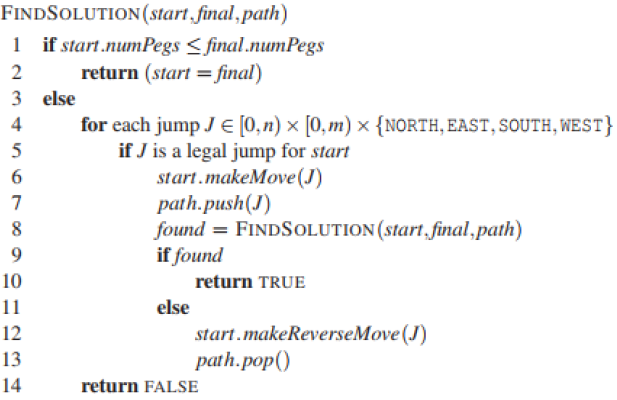
\includegraphics[width=1.0\textwidth,scale=1.0]{images/recursive_algorithm}
	\caption{Recurisve Algorithm \cite{lab5}}
\end{figure}

\section{Implementation}



\section{Theoretical Analysis}

\section{Results}

\section{Empirical Analysis}


\section{Conclusion}

\section{Group Member Contribution}

\section*{Acknowledgements}
I would like to Acknowledge the content and work from the Honours course Digital Image Processing (APPM4058A) lectured by Professor Sears. \\
All drawn diagrams were drawn using \url{http://draw.io/} and charts were made with Libre Office.\\ 
All the programming was done in python using NumPy and OpenCV libraries.\\


\bibliographystyle{plain}
\bibliography{biblio}{}

\end{document}